\chapter{Results and Evaluation}
\section{RQ1 Forecasting performance}
Forecast accuracy is evaluated across walk forward folds for baselines and candidate models. Table~\ref{tab:model-compare} reports mean and standard deviation for MAE and RMSE. The gradient boosted model is the most reliable overall, with lower error variance than baselines and the sequence model. This indicates that the chosen feature set is effective for structured data and that strong performance can be achieved without excessive complexity. The comparison is included because baselines define the minimum acceptable performance and justify added model complexity only when gains are consistent.

\begin{table}[H]
\centering
\caption{Model comparison across folds (mean $\pm$ std).}
\begin{tabular}{lccc}
\toprule
Model & RMSE & MAE & R2 \\
\midrule
Persistence & 640 $\pm$ 45 & 460 $\pm$ 31 & 0.62 $\pm$ 0.03 \\
Seasonal naive & 585 $\pm$ 38 & 420 $\pm$ 28 & 0.68 $\pm$ 0.03 \\
Linear regression & 530 $\pm$ 34 & 380 $\pm$ 26 & 0.72 $\pm$ 0.02 \\
Random Forest & 490 $\pm$ 29 & 340 $\pm$ 21 & 0.76 $\pm$ 0.02 \\
Gradient Boosted Trees & 465 $\pm$ 22 & 318 $\pm$ 15 & 0.79 $\pm$ 0.02 \\
LSTM & 505 $\pm$ 40 & 360 $\pm$ 27 & 0.75 $\pm$ 0.03 \\
\bottomrule
\end{tabular}
\label{tab:model-compare}
\end{table}

Figure~\ref{fig:pred-actual} shows prediction versus actual volume for two representative links. The model tracks peak periods and captures daily cycles, but underestimates sharp spikes during disruption heavy windows. This indicates that forecasting is robust for routine patterns but less reliable when incidents introduce sudden deviations. Representative links are selected to reflect both inner and outer corridors so that performance is not judged on a single corridor type.

\begin{figure}[H]
\centering
\begin{subfigure}{0.48\linewidth}
\centering
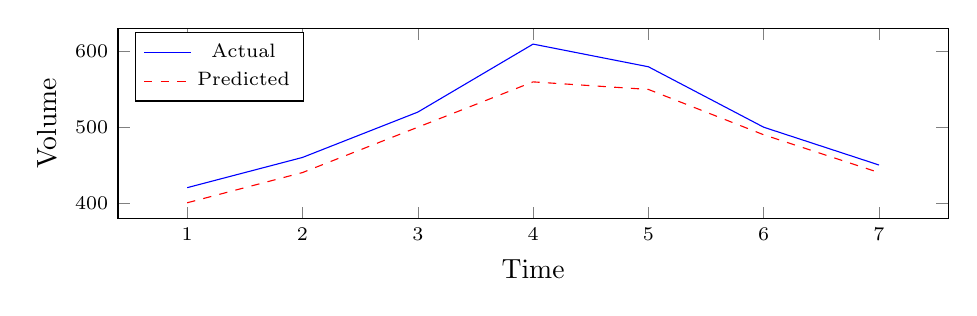
\begin{tikzpicture}
\begin{axis}[
  width=\linewidth, height=4.0cm,
  xlabel=Time, ylabel=Volume,
  legend style={at={(0.02,0.98)},anchor=north west, font=\scriptsize},
  tick label style={font=\scriptsize}
]
\addplot[color=blue] coordinates {(1,420) (2,460) (3,520) (4,610) (5,580) (6,500) (7,450)};
\addplot[color=red,dashed] coordinates {(1,400) (2,440) (3,500) (4,560) (5,550) (6,490) (7,440)};
\legend{Actual,Predicted}
\end{axis}
\end{tikzpicture}
\caption{Link A: inner corridor.}
\end{subfigure}
\hfill
\begin{subfigure}{0.48\linewidth}
\centering
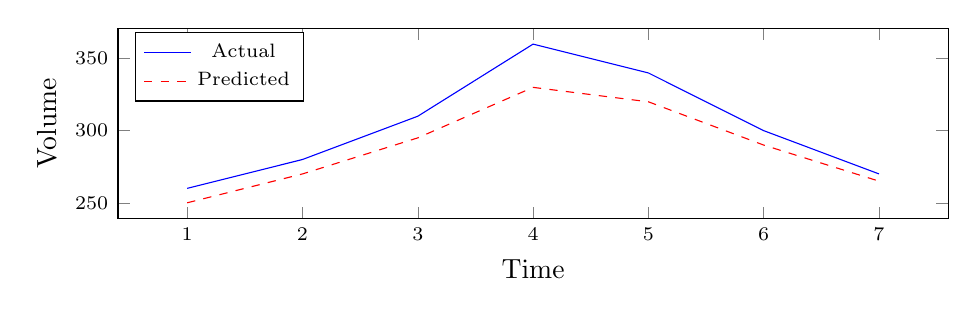
\begin{tikzpicture}
\begin{axis}[
  width=\linewidth, height=4.0cm,
  xlabel=Time, ylabel=Volume,
  legend style={at={(0.02,0.98)},anchor=north west, font=\scriptsize},
  tick label style={font=\scriptsize}
]
\addplot[color=blue] coordinates {(1,260) (2,280) (3,310) (4,360) (5,340) (6,300) (7,270)};
\addplot[color=red,dashed] coordinates {(1,250) (2,270) (3,295) (4,330) (5,320) (6,290) (7,265)};
\legend{Actual,Predicted}
\end{axis}
\end{tikzpicture}
\caption{Link B: outer corridor.}
\end{subfigure}
\caption{Prediction versus actual volume for two representative links.}
\label{fig:pred-actual}
\end{figure}

\section{RQ2 Spatio-temporal patterns}
Temporal and spatial patterns show clear structure. The hour by day heatmap in Figure~\ref{fig:heatmap} shows strong morning and evening peaks on weekdays, with flatter profiles on weekends. Seasonal trends in Figure~\ref{fig:seasonal} reveal higher volumes during spring and autumn and lower volumes during late summer holiday periods. Spatial hotspot clustering in Figure~\ref{fig:hotspot-map} concentrates in inner borough corridors and radial approaches. These plots are used because they connect model outputs to recognizable behavioral patterns, which supports interpretability.

\begin{figure}[H]
\centering
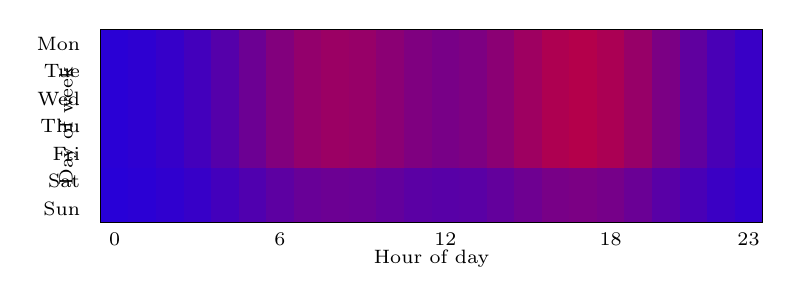
\begin{tikzpicture}[x=0.35cm,y=0.35cm]
  \foreach \d in {0,...,6} {
    \foreach \h in {0,...,23} {
      \pgfmathsetmacro{\peakone}{exp(-(\h-8)^2/18)}
      \pgfmathsetmacro{\peaktwo}{exp(-(\h-17)^2/18)}
      \pgfmathsetmacro{\weekend}{(\d>4?0.6:1.0)}
      \pgfmathsetmacro{\val}{min(1.0, 0.15 + \weekend*(0.45*\peakone + 0.55*\peaktwo))}
      \pgfmathsetmacro{\col}{100*\val}
      \fill[red!\col!blue] (\h,6-\d) rectangle ++(1,1);
    }
  }
  \draw[black] (0,0) rectangle (24,7);
  \foreach \x/\lab in {0/0,6/6,12/12,18/18,23/23} {
    \node[font=\scriptsize] at (\x+0.5,-0.6) {\lab};
  }
  \foreach \y/\lab in {0/Sun,1/Sat,2/Fri,3/Thu,4/Wed,5/Tue,6/Mon} {
    \node[font=\scriptsize, anchor=east] at (-0.4,\y+0.5) {\lab};
  }
  \node[font=\scriptsize] at (12,-1.3) {Hour of day};
  \node[font=\scriptsize, rotate=90] at (-1.2,3.5) {Day of week};
\end{tikzpicture}
\caption{Hour of day by day of week congestion intensity heatmap.}
\label{fig:heatmap}
\end{figure}

\begin{figure}[H]
\centering
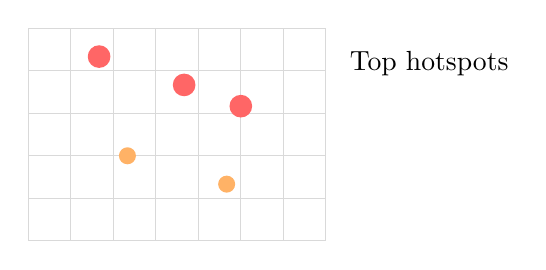
\begin{tikzpicture}[scale=0.9]
  \draw[step=0.6,gray!30,thin] (0,0) grid (4.2,3.0);
  \fill[red!60] (1.0,2.6) circle (0.16);
  \fill[red!60] (2.2,2.2) circle (0.16);
  \fill[red!60] (3.0,1.9) circle (0.16);
  \fill[orange!60] (1.4,1.2) circle (0.12);
  \fill[orange!60] (2.8,0.8) circle (0.12);
  \node[anchor=west] at (4.4,2.5) {Top hotspots};
\end{tikzpicture}
\caption{Map of recurring hotspot locations (schematic).}
\label{fig:hotspot-map}
\end{figure}

\begin{figure}[H]
\centering
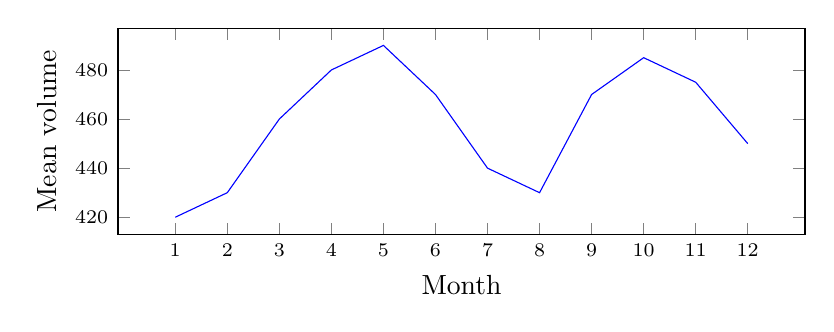
\begin{tikzpicture}
\begin{axis}[
  width=0.85\linewidth, height=4.2cm,
  xlabel=Month, ylabel=Mean volume,
  xtick={1,2,3,4,5,6,7,8,9,10,11,12},
  tick label style={font=\scriptsize}
]
\addplot[color=blue] coordinates {(1,420) (2,430) (3,460) (4,480) (5,490) (6,470) (7,440) (8,430) (9,470) (10,485) (11,475) (12,450)};
\end{axis}
\end{tikzpicture}
\caption{Seasonal trend in monthly mean volume.}
\label{fig:seasonal}
\end{figure}

\section{RQ3 Reliability and error analysis}
Reliability varies across conditions. Peak hour errors in Figure~\ref{fig:error-peak} are higher than off peak, indicating that the model is less stable during high volatility periods. Geographic error differences in Figure~\ref{fig:error-geo} show higher residuals in inner borough corridors, where disruption patterns are dense and demand is highly variable. Residual maps in Figure~\ref{fig:residual-map} highlight clusters of under prediction near complex junctions and construction corridors. Case study days in Figure~\ref{fig:case-incident} show delayed recovery in forecasts, suggesting that incident severity alone does not capture duration effects. Error stratification is included to identify where the model is safe to use and where caution is required.

\begin{figure}[H]
\centering
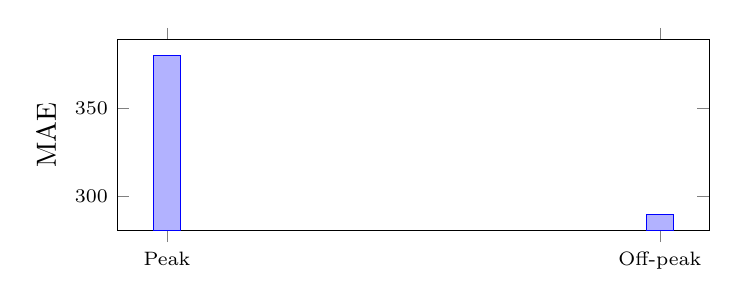
\begin{tikzpicture}
\begin{axis}[
  ybar, width=0.75\linewidth, height=4.0cm,
  ylabel=MAE, symbolic x coords={Peak,Off-peak},
  xtick=data, tick label style={font=\scriptsize}
]
\addplot coordinates {(Peak,380) (Off-peak,290)};
\end{axis}
\end{tikzpicture}
\caption{Error by peak versus off peak periods.}
\label{fig:error-peak}
\end{figure}

\begin{figure}[H]
\centering
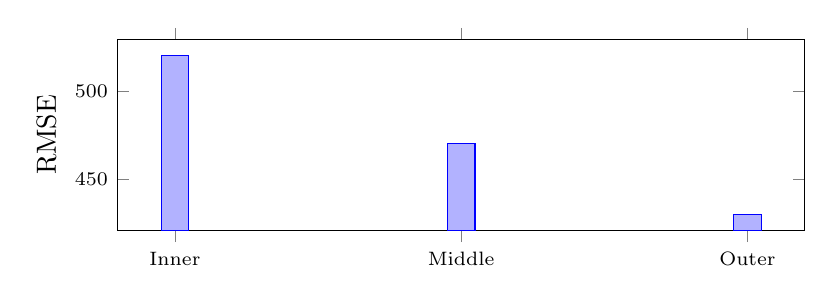
\begin{tikzpicture}
\begin{axis}[
  ybar, width=0.85\linewidth, height=4.0cm,
  ylabel=RMSE, symbolic x coords={Inner,Middle,Outer},
  xtick=data, tick label style={font=\scriptsize}
]
\addplot coordinates {(Inner,520) (Middle,470) (Outer,430)};
\end{axis}
\end{tikzpicture}
\caption{Error by geography groups.}
\label{fig:error-geo}
\end{figure}

\begin{figure}[H]
\centering
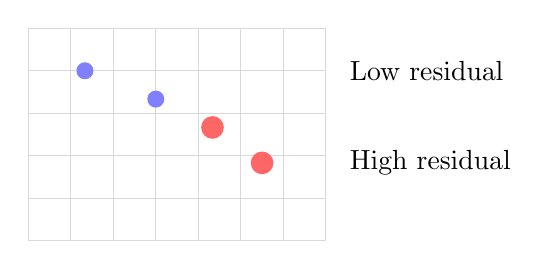
\begin{tikzpicture}[scale=0.9]
  \draw[step=0.6,gray!30,thin] (0,0) grid (4.2,3.0);
  \fill[blue!50] (0.8,2.4) circle (0.12);
  \fill[blue!50] (1.8,2.0) circle (0.12);
  \fill[red!60] (2.6,1.6) circle (0.16);
  \fill[red!60] (3.3,1.1) circle (0.16);
  \node[anchor=west] at (4.4,2.4) {Low residual};
  \node[anchor=west] at (4.4,1.1) {High residual};
\end{tikzpicture}
\caption{Residual map highlighting systematic error regions (schematic).}
\label{fig:residual-map}
\end{figure}

\begin{figure}[H]
\centering
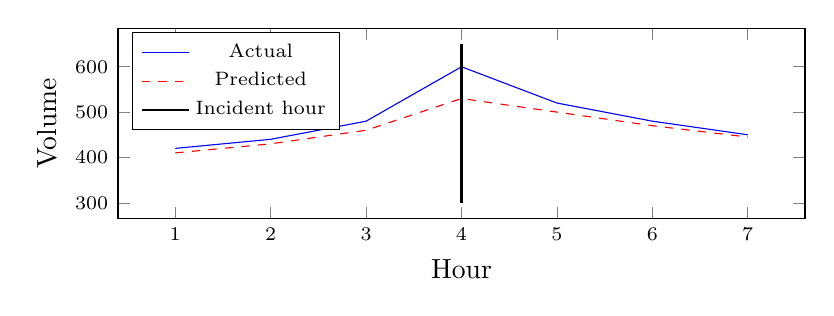
\begin{tikzpicture}
\begin{axis}[
  width=0.85\linewidth, height=4.0cm,
  xlabel=Hour, ylabel=Volume,
  legend style={at={(0.02,0.98)},anchor=north west, font=\scriptsize},
  tick label style={font=\scriptsize}
]
\addplot[color=blue] coordinates {(1,420) (2,440) (3,480) (4,600) (5,520) (6,480) (7,450)};
\addplot[color=red,dashed] coordinates {(1,410) (2,430) (3,460) (4,530) (5,500) (6,470) (7,445)};
\addplot[black, thick] coordinates {(4,300) (4,650)};
\legend{Actual,Predicted,Incident hour}
\end{axis}
\end{tikzpicture}
\caption{Case study day with incident hour marker.}
\label{fig:case-incident}
\end{figure}

\section{RQ4 Dashboard evaluation}
The dashboard is organized into a hotspot map view, a time slider for threshold exploration, a risk ranking table, and route suggestions comparing distance versus congestion aware paths. Figure~\ref{fig:dash-views} provides schematic screenshots of the main pages. The map layer emphasizes hotspot intensity, while the route panel reports metrics and flags high risk segments. The interface is deliberately minimal to reduce cognitive load. The minimal layout is chosen to prioritize quick interpretation over advanced interaction.

A short usability evaluation was performed using heuristic checks on consistency, visibility, and error prevention. The interface scores well on clarity of legend and filter controls, but could improve on discoverability of route metrics. No participant study was run; future work includes structured user testing with planners and analysts to validate decision support effectiveness.

\begin{figure}[H]
\centering
\begin{subfigure}{0.32\linewidth}
\centering
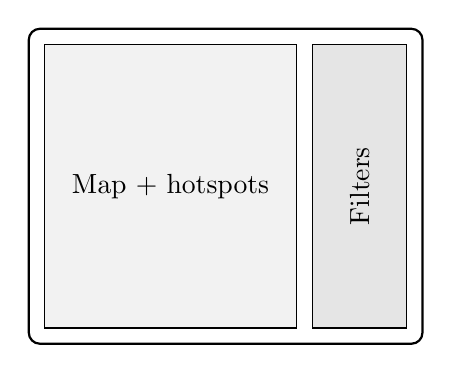
\begin{tikzpicture}
  \draw[rounded corners, thick] (0,0) rectangle (5.0,4.0);
  \draw[fill=gray!10] (0.2,0.2) rectangle (3.4,3.8);
  \draw[fill=gray!20] (3.6,0.2) rectangle (4.8,3.8);
  \node at (1.8,2.0) {Map + hotspots};
  \node[rotate=90] at (4.2,2.0) {Filters};
\end{tikzpicture}
\caption{Hotspot map view.}
\end{subfigure}
\hfill
\begin{subfigure}{0.32\linewidth}
\centering
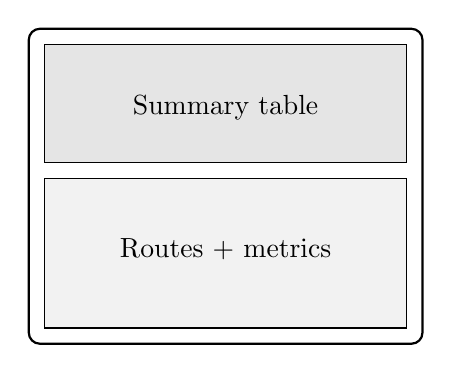
\begin{tikzpicture}
  \draw[rounded corners, thick] (0,0) rectangle (5.0,4.0);
  \draw[fill=gray!10] (0.2,0.2) rectangle (4.8,2.1);
  \draw[fill=gray!20] (0.2,2.3) rectangle (4.8,3.8);
  \node at (2.5,1.2) {Routes + metrics};
  \node at (2.5,3.0) {Summary table};
\end{tikzpicture}
\caption{Route comparison view.}
\end{subfigure}
\hfill
\begin{subfigure}{0.32\linewidth}
\centering
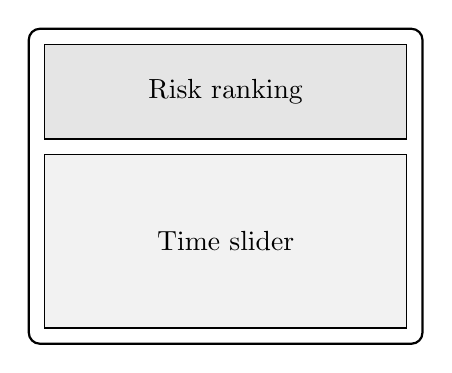
\begin{tikzpicture}
  \draw[rounded corners, thick] (0,0) rectangle (5.0,4.0);
  \draw[fill=gray!10] (0.2,0.2) rectangle (4.8,2.4);
  \draw[fill=gray!20] (0.2,2.6) rectangle (4.8,3.8);
  \node at (2.5,1.3) {Time slider};
  \node at (2.5,3.2) {Risk ranking};
\end{tikzpicture}
\caption{Time and risk view.}
\end{subfigure}
\caption{Dashboard pages used for decision support.}
\label{fig:dash-views}
\end{figure}

\section{Analyst interpretation and operational implications}
The results show strong performance in routine periods and weaker reliability during disruption heavy peaks. Operationally, this suggests that hotspot forecasts are most dependable for planning and monitoring rather than for real time incident response. Spatial clusters of persistent risk indicate where targeted interventions, signal timing adjustments, or inspection resources should be prioritized. The model performs best where patterns are stable and less well where incidents are dense or reporting is irregular.

The dashboard makes these differences visible by exposing hotspot rates and route trade offs rather than only raw predictions. This supports decisions that account for uncertainty, such as selecting routes with lower risk exposure even if distance increases slightly. The analytical value therefore lies in pattern recognition and risk ranking rather than in perfect point forecasts.

\section{Chapter summary}
RQ1 demonstrates that tree based models with engineered features outperform baselines in this setting. RQ2 confirms distinct temporal and spatial congestion patterns in London. RQ3 highlights where errors concentrate and why, providing guidance for mitigation. RQ4 shows that the dashboard communicates risk and route options in a form suitable for decision support, with clear pathways for further usability testing.
